\chapter{Приложение}

В приложении мы рассмотрим пример системы, состоящей из случайного процесса с выходом в сток, функционирующим с учётом глобального условия на достижимость.
Мы воспользуемся теоремой из первого предложенного подхода для расчёта предельного состояния системы, а также получим её состояния на разных промежутках времени с помощью программной реализации вычислительного подхода. После этого мы визуализируем результаты и сможем убедиться, что спустя продолжительное время результаты обоих подходов сходятся. 

Пусть задан ориентированный граф $G$, представленный на рис.\ref{fig:pic_4}:

\begin{figure}
	\centering	
	{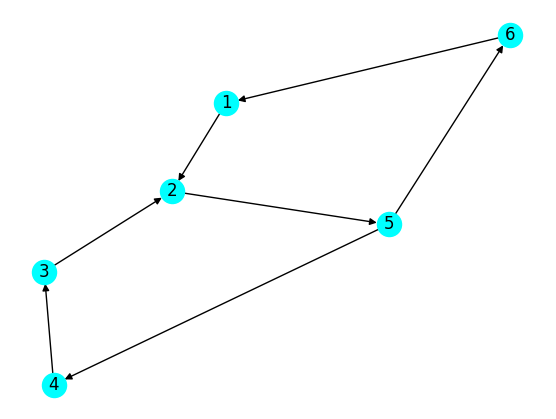
\includegraphics[width=0.8\textwidth]{img/4.png}}
	{Граф $G$}
	\label{fig:pic_4}
\end{figure}

Переходы по всем его дугам равновероятны, и таким образом он задаёт случайный процесс. Положим $p = 2$ и назначим вершину 2 выходной. Его вспомогательный граф $G'$, состоящий из двух изолированных сильно связных компонент (без стока), показан на рис.\ref{fig:pic_5}:

\begin{figure}
	\centering	
	{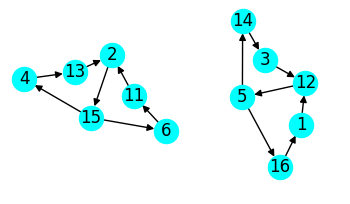
\includegraphics[width=0.9\textwidth]{img/5.png}}
	{Граф $G'$}
	\label{fig:pic_5}
\end{figure}

Этот граф --- 4-циклический, и значит, у нас нет взаимной простоты длин контуров и параметра $p$. Используя размышления из наивного подхода, получаем, что множество вершин графа $G$ разбивается на $X_{in} = \{1, 3, 5\}$ и $X_{out} = \{2, 4, 6\}$. Частицы, начавшие перемещаться из вершин первого множества, останутся циркулировать по графу, а остальные покинут его в пределе. 

Рассмотрим три разных начальных распределения частиц по вершинам и приведём графики, отражающие их расположение на разных временных этапах, а также график количества частиц, покинувших граф, по времени. 

\newpage

\begin{example}
	Распределение частиц: $\{1: 6, 2: 0, 3: 0, 4: 3, 5: 11, 6: 0\}$
	
	\begin{figure}
		\centering	
		{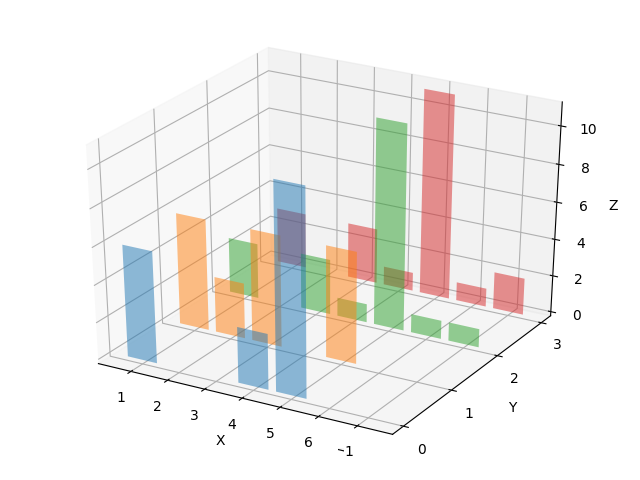
\includegraphics[width=0.7\textwidth]{img/e1.png}}
		{Распределение частиц по вершинам}
		\label{fig:pic_e1}
	\end{figure}

	\begin{figure}
		\centering	
		{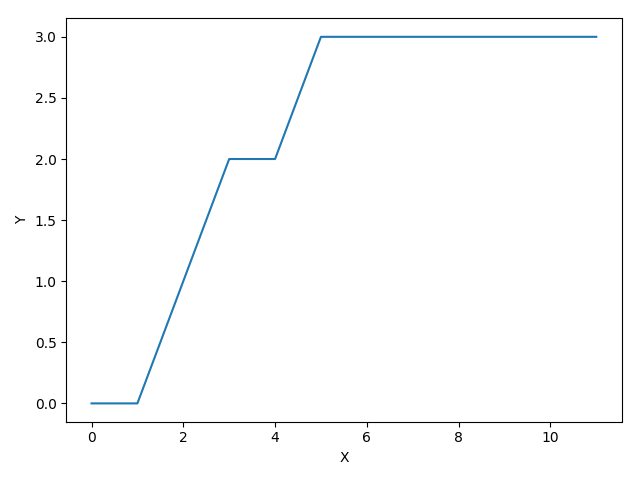
\includegraphics[width=0.7\textwidth]{img/e11.png}}
		{Количество частиц в стоке}
		\label{fig:pic_e11}
	\end{figure}
	
\end{example}

\newpage

\begin{example}
	Распределение частиц: $\{1: 6, 2: 0, 3: 0, 4: 3, 5: 11, 6: 0\}$
	
	\begin{figure}
		\centering	
		{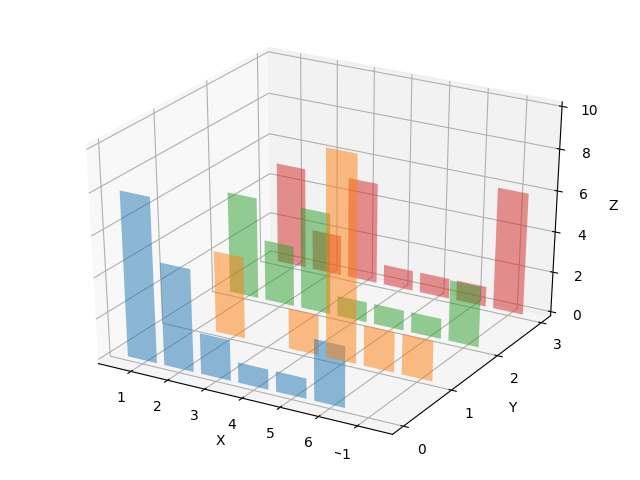
\includegraphics[width=0.7\textwidth]{img/e2.png}}
		{Распределение частиц по вершинам}
		\label{fig:pic_e2}
	\end{figure}
	
	\begin{figure}
		\centering	
		{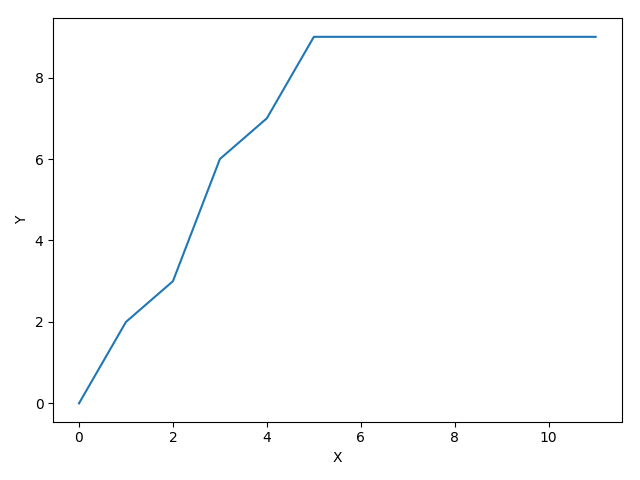
\includegraphics[width=0.7\textwidth]{img/e22.png}}
		{Количество частиц в стоке}
		\label{fig:pic_e22}
	\end{figure}
	
\end{example}

\newpage

\begin{example}
	Распределение частиц: $\{1: 3, 2: 1, 3: 10, 4: 1, 5: 5, 6: 0\}$
	
	\begin{figure}
		\centering	
		{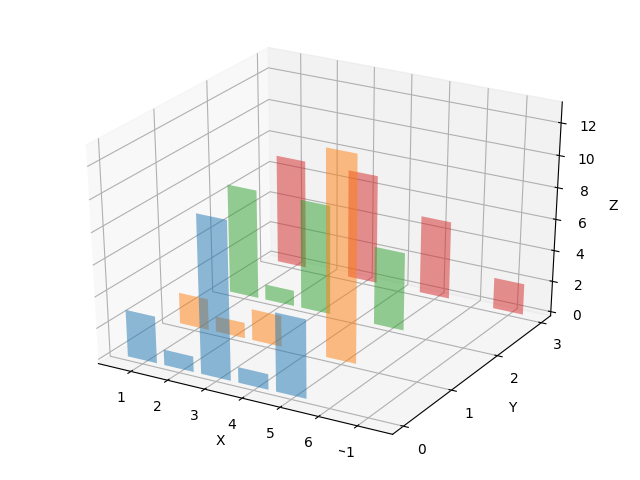
\includegraphics[width=0.7\textwidth]{img/e3.png}}
		{Распределение частиц по вершинам}
		\label{fig:pic_e2}
	\end{figure}
	
	\begin{figure}
		\centering	
		{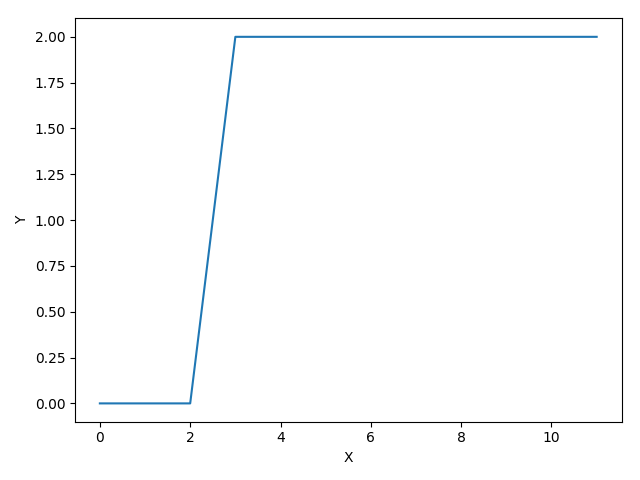
\includegraphics[width=0.7\textwidth]{img/e33.png}}
		{Количество частиц в стоке}
		\label{fig:pic_e22}
	\end{figure}
	
\end{example}

На верхних графиках по оси $x$ пронумерованы вершины и -1 --- сток; по $y$ --- $\log_2(t)$, где $t$ --- рассматриваемый такт времени, и по $z$ --- количество частиц в соответствующей вершине. Нижние графики отображают зависимость количества частиц в стоке по оси $y$ от такта времени (тоже в виде логарифма) по $x$. Изначально по вершинам распределяется 20 частиц.

Как видим, во всех примерах уже по истечению первых ста тактов граф покидают все частицы, изначально расположенные в вершинах из $X_{out}$, и продолжает циркулировать постоянное количество частиц, которые стартовали в вершинах множества $X_{in}$, как раз в соответствии с нашими рассуждениями.



